% !TEX root = ../../../main/aws_chabauty.tex
\newpage
\section{Bas Edixhoven: Geometric Quadratic Chabauty}
\subsection{Lecture 1}

This is joint work with Guido Lido. Let $C/\Q$ be a `nice' curve with genus $g>1$, and assume that we have a rational point $b \in C(\Q)$. We have a map $j_b: C \to J$ given by $P \mapsto O_C(P-b)$. The Chabauty method has a problem if $r \not<g$:
	\[
	\begin{tikzcd}
	C(\Q) \arrow{r} \arrow{dd} & J(\Q) \arrow[draw=none]{d}[sloped,auto=false]{\subseteq} \\
	&  \ov{J(\Q)} \arrow[draw=none]{d}[sloped,auto=false]{\subseteq} \\
	C(\Qp) \arrow{r} & J(\Qp) 
	\end{tikzcd}
	\]
Our idea is to replace $J$ be something bigger, of higher dimension, and then play the Chabauty `game'.


The question is, what object to take? A $\G_m$-torsor (line bundle minus 0-section). Given the map $j_b: C \to J$, we have a diagram

	\begin{figure}[!ht]
	\centering
	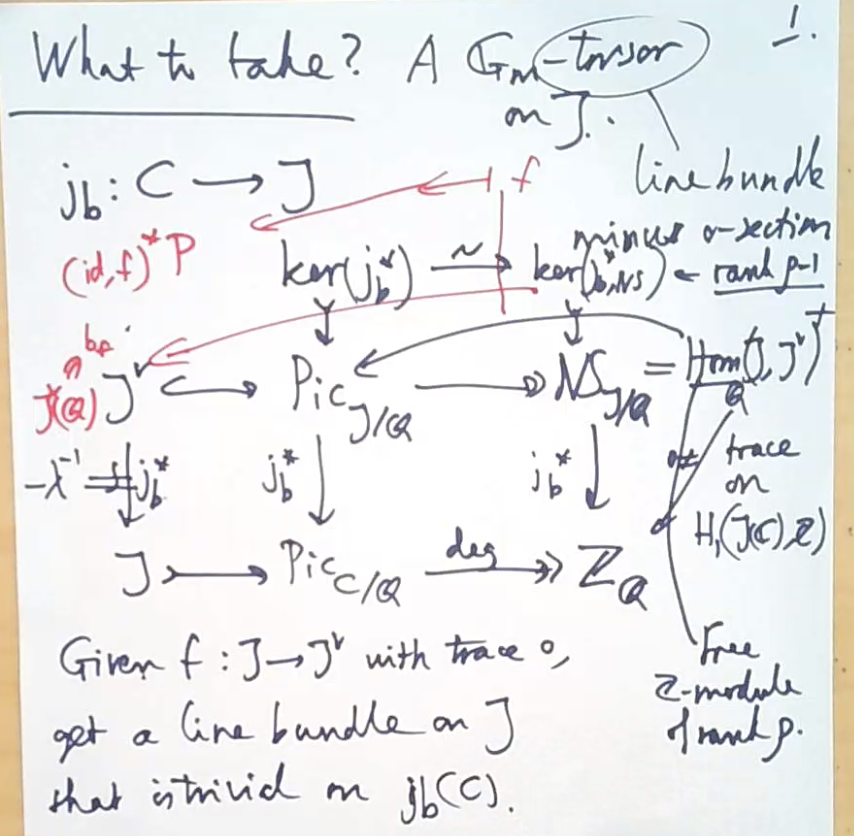
\includegraphics[width=0.5\textwidth]{../images/im5.png}
	\end{figure}


% Poincare Bundle
\subsection{Poincar\'e Bundle}

For all abelian varieties $A$, we can view $A^\vee$ as $\ext^1(A,\G_m)$, where
	\[
	\G_m \ma{} E \ma{\G_m \text{ torsor}} A
	\]
The maps $\G_m \to E$ are rigid: they have no non-trivial automorphisms that induce $\id_A$ and $\id_{\G_m}$. So over $A^\vee$, we have a universal extension 
	\[
	\begin{tikzcd}
	\G_{m,A} \arrow[hook]{r} \arrow{dr} & P^\times \arrow{d} \arrow[two heads]{r} &  A \times A^\vee \arrow{dl} \\
	& A^\vee & 
	\end{tikzcd}
	\]
$P^\times$ is also the universal extension of $A^\vee$ by $\G_m$ over $A$. So we have
	\[
	\begin{tikzcd}
	j_b^* T_{f} \arrow{r} \arrow{d} & T_{f \; r} \arrow{r} & P^\times \arrow{d} \\
	C \arrow{r}{j_b} \arrow{u} \arrow{ur}{j_b} & J \arrow{r}{(\id, \text{tr}_{b_f} \circ f)} & J \times J^\vee
	\end{tikzcd}
	\]
We know $J$ has dimension $g$ and $T_{f r}$ has dimension $g+1$. Take a $\Z$-basis $f_1, \ldots, f_{j-1}$ of $\ker(j_{b??}^*)$, gives
	\[
	\begin{tikzcd}
	& T \arrow{r} \arrow{d} &  (P^\times)^{j-1} \arrow{d} \\
	C \arrow{r}{j_b} \arrow{ur}{\tilde{j}_b} & J \arrow{r}{(\id,\tr_{b_{f_1}} \circ f_1, \ldots, \tr_{b_{f_1}})} & J \times (J^\vee)^{p-1} 
	\end{tikzcd}
	\]
Now $(P^\times)^{j-1}$ is a $\G_m^{p-1}$ torsor and $T$ has dimension $g+p-1$. We play the Chabauty game in $T$. We hope that if it works that $r< g+p-1$. (most wanted example have $p= g$). Now $T(\Q)$ is a $\Q^{\times,p-1}$-torsor.
	\[
	\begin{tikzcd}
	T(\Q) \arrow{d} \\
	J(\Q)
	\end{tikzcd}
	\]
Now $\Q^\times= \{\pm 1\} \times \Z$ (set of primes). There is a big problem: there are too many $\Q$-points in $T$. As a solution, we extend the geometry over $\Z$, $\Z^\times= \{\pm1\}$. 


\begin{rem}
{\bfseries From now on, everything is over $\Z$}
\end{rem}


Let $C$ be a proper, regular model of $C_\Q$, and let $J$ be the N\'eron model of $J_\Q$. Let $J^\vee$ be the N\'eron model of $J_\Q^\vee, J^{\vee,0} \subset J^\vee$, is the fiberwise connected component of $\alpha$. Now $P^\times$ is the unique extension of $P^\times_\Q$ to $J \times J^{\vee,0}$ as a bi-extension.


Now $P^\times$ is a $\G_m$-biextension of $A \times A^\vee$. Then there are two partial group laws, given by what we have already seen. For example, one of them is: if $x_1,x_2 \in A$, and $y \in A^\times$, i.e. $(x_1,y),(x_2,y) \in A \times A^\vee$, $z_1 \in P^\times(x_1,y)$, $z_2 \in P^\times(x_2,y)$, then we obtain $z_1 +_1 z_2 \in P^\times(x_1+x_2,y)$. 


We use the biextension structure of $P^\times$ over $J \times J^{\vee,0}$ to parametrize 
	\[
	\begin{tikzcd}
	T(\Z) \arrow{d} \\
	J(\Z) \arrow[bend left=40, dotted]{u}
	\end{tikzcd}
	\]
noting that $T(\Z)$ is a $(\pm 1)^{p-1}$-torsor. 
	\[
	\begin{tikzcd}
	C(\Z) \arrow{dd} \arrow{r} & T(\Z) \arrow[draw=none]{d}[sloped,auto=false]{\subseteq} \\
	& \ov{T(\Z)} \arrow[draw=none]{d}[sloped,auto=false]{\subseteq} \\
	C(\Z_p) \arrow{r} & T(\Z_p) 
	\end{tikzcd}
	\]
Now $C(\Z_p)$ is 1-dimensional, $g+p-1$-dimensional, and $\ov{T(\Z)}$ is at most $r$-dimensional. 

















 